\begin{block}{Notation}
\large
    \begin{itemize}
        \itembox{$\pspace \subset \RR^P$} Parameter Space
        \itembox{$\obs: \pspace \to \mathcal{O} \subset \RR^D$} Observables
        \itembox{$\nspace \subset \RR^D$} Noise Space
        \itembox{$\param^\dagger\in\pspace$} True Parameter
        \itembox{$\data(\noise) \subset \RR^D$} Possible Data, $d_i(\noise) = \obs_i(\param^\dagger) + \xi_i$
        \itembox{$\noise^\dagger\in\nspace$} Noise in Measurements
        \itembox{$ \sigma $} Variance of Noise
        \itembox{$\data^\dagger\in\RR^D$} Observed Data, $\data^\dagger = \data(\noise^\dagger)$
    \end{itemize}

\end{block}

%\begin{block}{Quantity of Interest Map}
\centering
\vspace{1cm}
\heading{\Large Quantity of Interest Map}
\vspace{1cm}
    \emph{\large Defines a (functional) relationship between predictions and data}

        $$Q \left (\param, \noise \right ) = F \left ( \obs(\param), \data(\noise) \right ) $$
        $$Q \left (\param \right ) = F \left ( \obs(\param), \data^\dagger \right )$$
        $$Q \left ( \pspace, \nspace \right ) =: \dspace_\mathcal{T} \subset \RR$$
        $$Q \left ( \pspace \right ) =: \dspace_\mathcal{C} \subset \dspace_\mathcal{T}$$

    \begin{figure}
        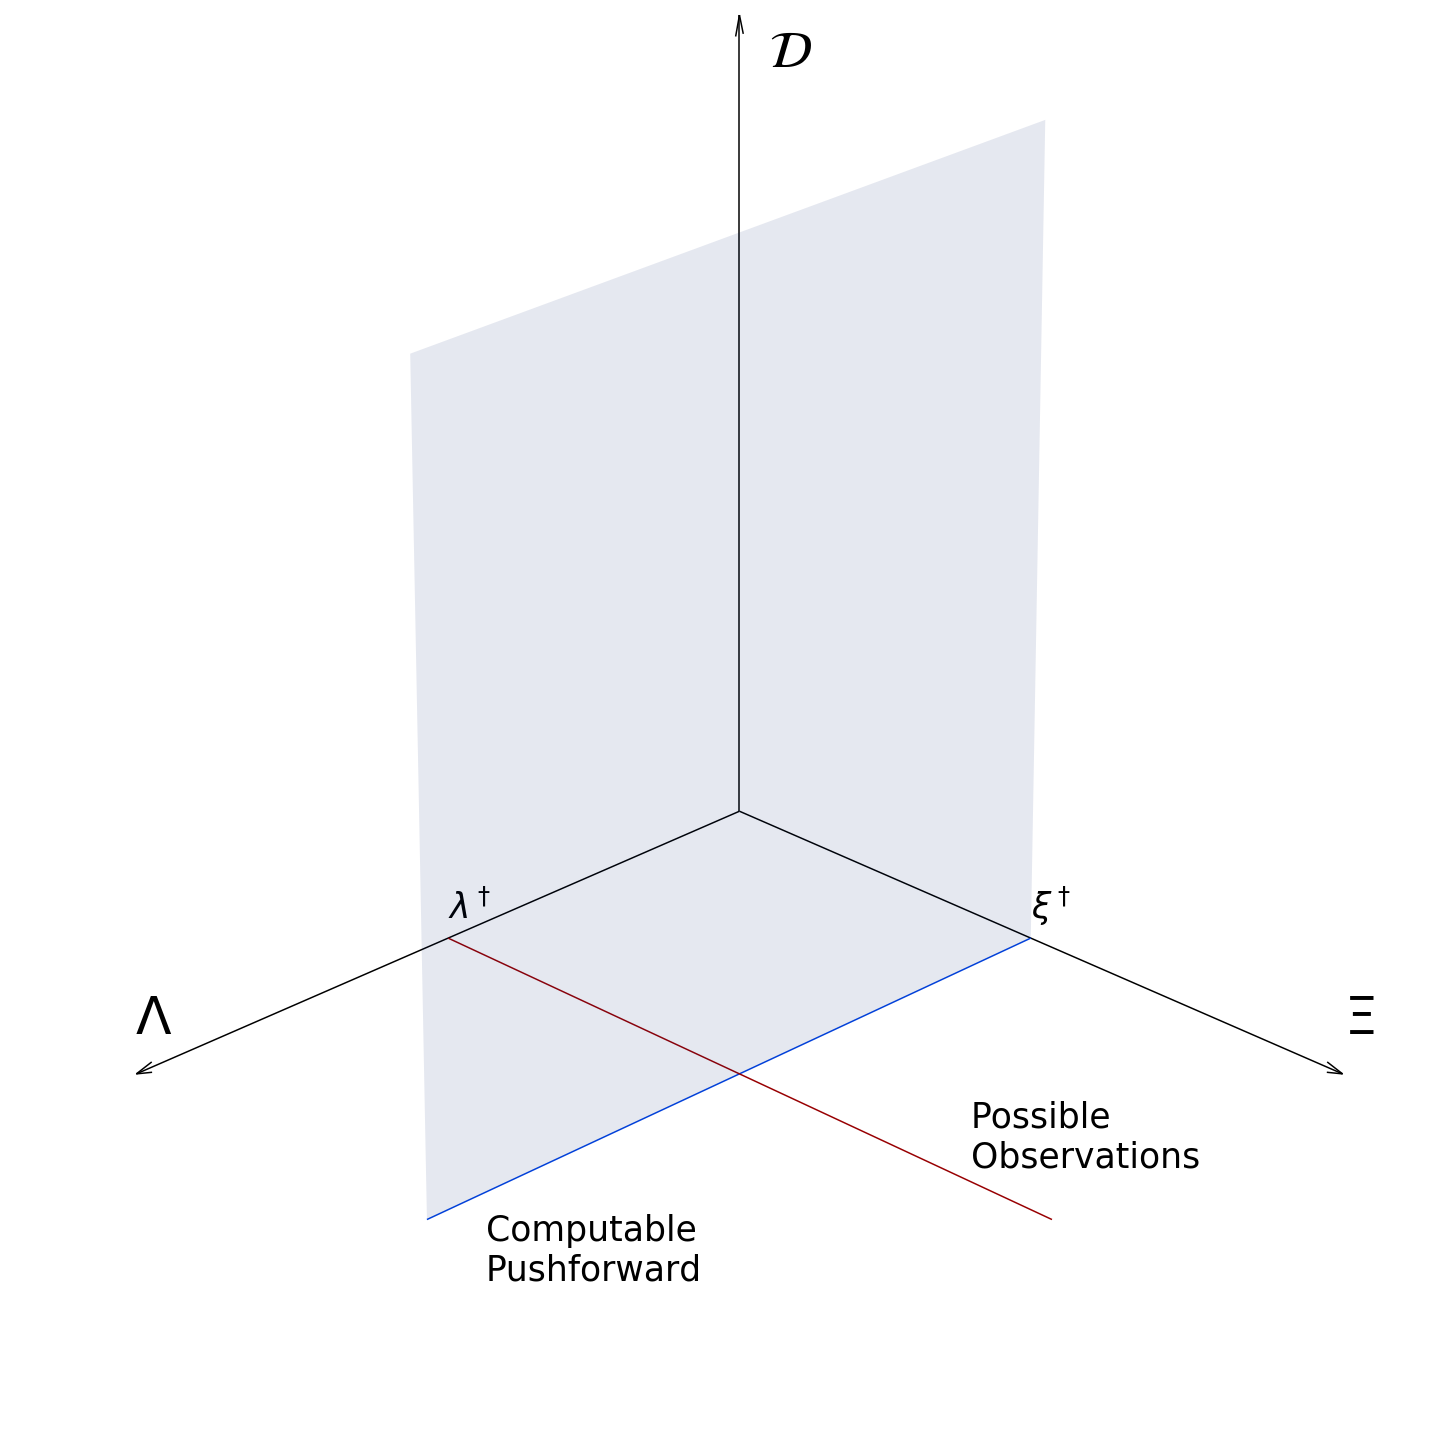
\includegraphics[height=27cm]{diagram}
    \caption*{\large \emph How do conditionals of $\nspace$ compare to the joint density?}
    \end{figure}

%\end{block}
